\let\negmedspace\undefined
\let\negthickspace\undefined
\documentclass[journal]{IEEEtran}
\usepackage[a5paper, margin=10mm, onecolumn]{geometry}
%\usepackage{lmodern} % Ensure lmodern is loaded for pdflatex
\usepackage{tfrupee} % Include tfrupee package

\setlength{\headheight}{1cm} % Set the height of the header box
\setlength{\headsep}{0mm}     % Set the distance between the header box and the top of the text

\usepackage{gvv-book}
\usepackage{gvv}
\usepackage{cite}
\usepackage{amsmath,amssymb,amsfonts,amsthm}
\usepackage{algorithmic}
\usepackage{graphicx}
\usepackage{textcomp}
\usepackage{xcolor}
\usepackage{txfonts}
\usepackage{listings}
\usepackage{enumitem}
\usepackage{mathtools}
\usepackage{gensymb}
\usepackage{comment}
\usepackage[breaklinks=true]{hyperref}
\usepackage{tkz-euclide} 
\usepackage{listings}
\def\inputGnumericTable{}                                 
\usepackage[latin1]{inputenc}                                
\usepackage{color}                                            
\usepackage{array}                                            
\usepackage{longtable}                                       
\usepackage{calc}                                             
\usepackage{multirow}                                         
\usepackage{hhline}                                           
\usepackage{ifthen}                                           
\usepackage{lscape}
\begin{document}

\bibliographystyle{IEEEtran}
\vspace{3cm}

\title{1.7.5}
\author{AI25BTECH11019 - MENAVATH SAI SANJANA}
% \maketitle
% \newpage
% \bigskip
{\let\newpage\relax\maketitle}

\renewcommand{\thefigure}{\theenumi}
\renewcommand{\thetable}{\theenumi}
\setlength{\intextsep}{10pt} % Space between text and floats


\numberwithin{equation}{enumi}
\numberwithin{figure}{enumi}
\renewcommand{\thetable}{\theenumi}

\textbf{Question}:\\
 Find the value of p for which the points (-5,1),(1,p),(4,-2) are collinear 
\\
\bigskip
\textbf{Solution: }

Let the points be

\begin{table}[h!]
\centering
\begin{tabular}{|c|c|}
\hline
\textbf{Point} & \textbf{Name} \\
\hline
$\myvec{-5 \\ 1}$ & $\vec{A}$ \\
\hline
$\myvec{1 \\ p}$ & $\vec{B}$ \\
\hline
$\myvec{4 \\ -2}$ & $\vec{C}$ \\
\hline
\end{tabular}
\caption{Variables Used}
\end{table}



The difference vectors are
\begin{align}
(\vec{B}-\vec{A}) &= \myvec{6 \\ p-1}, \\
(\vec{C}-\vec{A}) &= \myvec{9 \\ -3}.
\end{align}

Thus,
$
M^T = (\vec{B}-\vec{A} \;\; \vec{C}-\vec{A})^T
= \myvec{6 & p-1 \\ 9 & -3}.
$

Apply row operations to convert $M^T$ into upper triangular form.

\begin{align}
\myvec{6 & p-1 \\ 9 & -3} 
&\xrightarrow{R_2 \to R_2 - \tfrac{3}{2}R_1}
\myvec{6 & p-1 \\ 0 & -\tfrac{3}{2}(p+1)}.
\end{align}

For collinearity, $\operatorname{rank}(M^T)=1$.  
This happens when the second row is zero:
$
-\tfrac{3}{2}(p+1)=0.
$

$
p = -1
$

\bigskip

\textbf{Hence, the three points $A,B,C$ are collinear when $p=-1$.}

\begin{figure}[ht!]
    \centering
    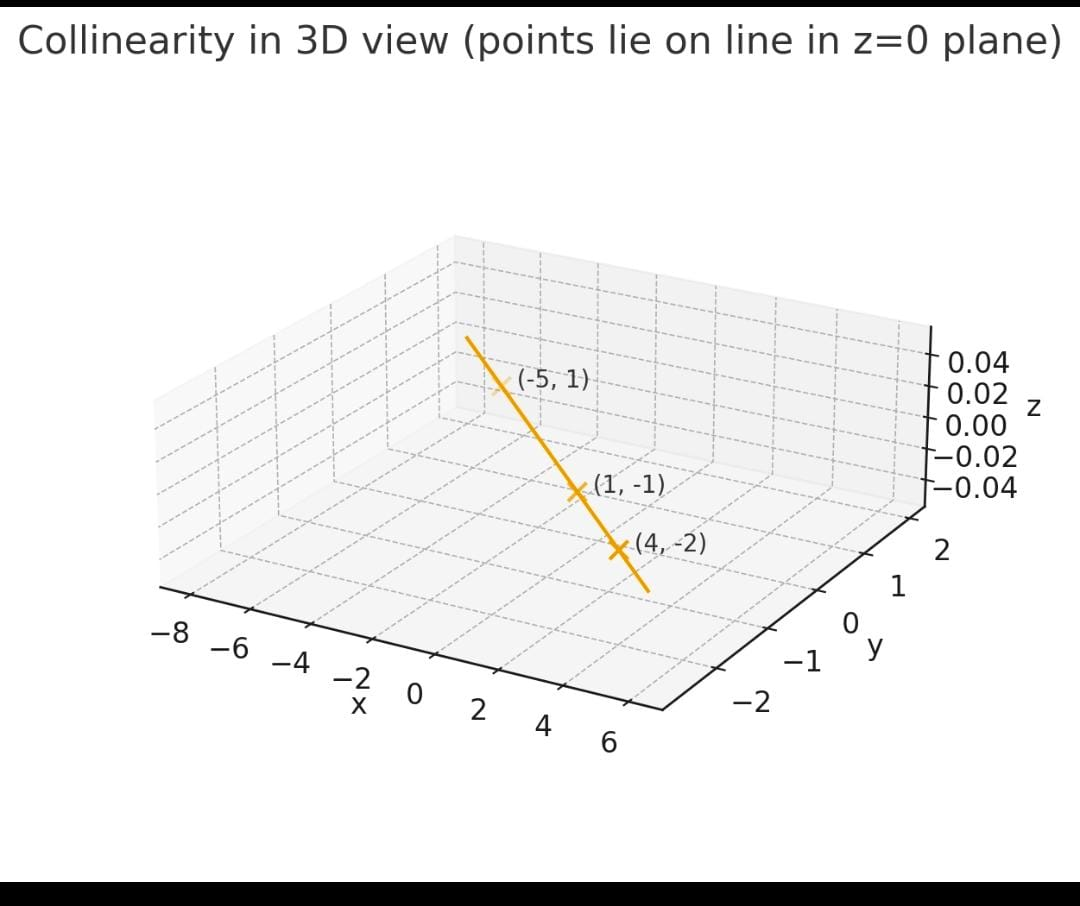
\includegraphics[width=0.9\textwidth]{figs/matgeo-1.7.5.jpeg}
    \caption{}
    \label{fig:1.2.27.jpg}
\end{figure}

\end{document}
